\documentclass[12pt,a4paper,ngerman]{article}
\usepackage[german,ngerman]{babel} % sorgt dafür, dass "Inhaltsverzeichnis" auf deutsch angezeigt wird, und wahrscheinlich noch ein paar andere Sachen auch


% alles bezüglich Matheformeln

% Gleichungen linksbündig
\usepackage[fleqn]{amsmath}

% wieweit Gleichungen vom linken Rand aus abgerückt werden
\setlength\mathindent{20pt}

\usepackage{amsmath}
\usepackage{amsfonts}
\usepackage{amssymb}

% Schriftart ohne Serifen für Formeln
\usepackage{cmbright}
%\SetSymbolFont{largesymbols}{normal}{OMX}{iwona}{m}{n}

\usepackage{mathtools}


% Seitenlayout (Ränder)
\usepackage[top=2.5cm, bottom=2.5cm, outer=4cm, inner=2.5cm, heightrounded, marginparwidth=2.5cm, marginparsep=0.5cm]{geometry}

% Bildunterschriftdesign
\usepackage[font=small,labelfont=bf]{caption}
\usepackage{caption}



\usepackage{graphicx}



% Benutzerdefinierte Farben
\usepackage{color}
\definecolor{light-gray}{gray}{0.95}

% ermöglicht eine Ausrichtung von Text am & Zeichen
\usepackage{tabularx}

\usepackage{xparse}
\ExplSyntaxOn
\NewDocumentEnvironment{benannteAuflistung} { oo }
	{
		\IfValueTF{#2}
		{
			\tabularx{\textwidth} {@{\hspace{0.0cm}} #2 @{}}
			\IfValueTF{#1}
	    	{
			   	\multicolumn{2}{@{\hspace{0.0cm}}l}{\textbf{#1}}  \\
	     	}
			{
			}
		}
		{
			\tabularx{\textwidth} {@{\hspace{0.0cm}} lX @{}}
			\IfValueTF{#1}
	    	{
			   	\multicolumn{2}{@{\hspace{0.0cm}}l}{\textbf{#1}}  \\
	     	}
			{
			}
		}
    }
    {
    	\endtabularx
    }
\ExplSyntaxOff




% Schriftart für SourceCodeListings
%\usepackage{sourcecodepro}

% Programmcode Formatierung
\usepackage{listings}
\lstset{
	backgroundcolor=\color{light-gray},
	breaklines=true,
	captionpos=b,
	frame=none, % zB leftline oder single
	keepspaces=true,
	keywordstyle=\color{olive},
	%numbers=left,
	numbersep=5pt,
	tabsize=4,
	%numberstyle=\tiny,
    basicstyle=\footnotesize %\ttyfamily
}

% Kopf- und Fußzeile
\usepackage[headsepline,footsepline]{scrpage2}
\pagestyle{scrheadings}
\clearscrheadfoot

% Kopfzeile
\ihead{Hochschule München - Segway}
\ohead{\headmark}
\automark[subsection]{section}

%Fußzeile
\ifoot{\autoren}
\ofoot{\pagemark}


% hiermit kann man später angeben, wer welche Seite geschrieben hat
\newcommand{\autoren}{}
















\usepackage{wrapfig, ragged2e}

\usepackage{float}
\usepackage{fontspec,xunicode}  % dadurch kann man auch äöü direkt im text eingeben



\usepackage[utf8]{inputenc}



% sollte eigentlich Gleichungen linksbündig ausrichten
%\def\changemargin#1#2{\list{}{\rightmargin#2\leftmargin#1}\item[]}
%\let\endchangemargin=\endlist

%\newfontfamily\codefont[]{Hack}
%\lstset{basicstyle=\codefont,breaklines=true}

% sorgt dafür, dass nicht so viel Platz über und unter Gleichungen eingefügt wird
\newenvironment{mathezeug}
 {\setlength{\abovedisplayskip}{00pt}\setlength{\belowdisplayskip}{\baselineskip}}%
 %\csname flalign*\endcsname}
 %{\csname endflalign*\endcsname\ignorespacesafterend}


\newcommand\tab[1][1cm]{\hspace*{#1}}


\setmainfont{Arial}

\setcounter{secnumdepth}{4} % erlaubt Unter-Unter-Kapitel

% folgendes macht automatisch Links im Inhaltsverzeichnis des Pdfs, die direkt zum Unterkapitel führen
\usepackage[colorlinks,pdfpagelabels,pdfstartview = FitH,bookmarksopen = true,
bookmarksnumbered = true,linkcolor = black,plainpages = false,hypertexnames = false,
citecolor = black] {hyperref}


% für Zitate
\usepackage[style=numeric, backend=bibtex]{biblatex}
\addbibresource{Quellenverzeichnis}  % Bibtex-Datei wird schon in der Preambel eingebunden

% Sachen wegen Literaturverzeichnis
\usepackage{url}
\newcommand*\oldurlbreaks{}
\let\oldurlbreaks=\UrlBreaks
\renewcommand{\UrlBreaks}{\oldurlbreaks\do\\}
%\renewcommand{\UrlBreaks}{\oldurlbreaks\do\a\do\b\do\c\do\d\do\e%
%  \do\f\do\g\do\h\do\i\do\j\do\k\do\l\do\m\do\n\do\o\do\p\do\q%
%  \do\r\do\s\do\t\do\u\do\v\do\w\do\x\do\y\do\z\do\?\do\&}
\usepackage{hyperref}


\usepackage[disable]{todonotes}

%\raggedright % verhindert Blocksatz

% Zeilenabstand = 1.5
\usepackage{setspace}
\onehalfspacing









\begin{document}
\setlength{\parindent}{0pt} % kein Einzug bei Absatzanfang
\captionsetup{singlelinecheck=false}
% !TEX root = SegwayDoku.tex

\begin{titlepage}
\thispagestyle{empty}
\newgeometry{left=3cm,bottom=2cm, outer=2cm, top=2cm}
\begin{flushleft}
\begin{Huge}
\textbf{Hochschule München}
\par\medskip
Projektarbeit Wackelroboter
\end{Huge}
\begin{large}
\par\vspace{5cm}
\begin{figure}[h]
\centering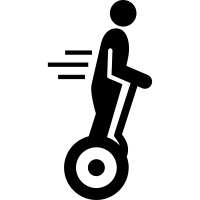
\includegraphics[width=0.3\textwidth]{images/segwayIcon.png}

% würde eine Bildunterschrift erzeugen
%\caption[Eintrag im Abbildungsverzeichnis]{}
\end{figure}

\par\vspace{5cm}

\begin{large}
\begin{tabbing}
Betreuer \hspace{2cm}\= Prof. Dr. Norbert Nitzsche \\\\
Verfasser \> Valentyn Chepil, Stephan Morongowski, \\ \> Severin Schendel, Aleksandar Stoiljkovic, Timo Veit \\
%Adresse \> Hauptstraߟe 45 - 85293 Reichertshausen \\
%Telefon \> 0176-23837636 \\
Fachbereich \> Maschinenbau - MBB \\
Abgabetermin \> 28.2.2018

\end{tabbing}
\end{large}




\end{large}
\end{flushleft}


%\centering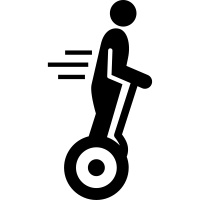
\includegraphics{images/segwayIcon.jpg}
\vfill % Fill the rest of the page with whitespace
\end{titlepage}
\restoregeometry




%\pdfbookmark[1]{Inhaltsverzeichnis}{toc}

% verhindert die Fuߟzeile für die aktuelle Seite
\thispagestyle{empty}

\tableofcontents
\newpage
\thispagestyle{empty}
\listoffigures
\newpage
\setcounter{page}{1}


% hier werden alle Extradateien eingebunden
% !TEX root = test.tex
\renewcommand{\autoren}{Aleksandar Stoiljkovic}

\section{Motivation}
Warum wir einen Roboter bauen wollen.
\par\bigskip
Finster war's, der Mond schien helle auf die grünbeschneite Flur, als
ein Wagen blitzesschnelle langsam um die runde Ecke fuhr. Drinnen
saßen stehend Leute schweigend ins Gespräch vertieft, als ein
totgeschossner Hase auf dem Wasser Schlittschuh lief und ein
blondgelockter Knabe mit kohlrabenschwarzem Haar auf die grüne Bank
sich setzte, die gelb angestrichen war.
\newpage

% !TEX root = Beispielhauptdokument.tex
\renewcommand{\autoren}{Stephan Morongowski}
\newpage
\section{Navigation}

Wie navigiert man in der Ebene? Hier ein Beispiel für ein Zitat: Wie in \cite{bildungAtmosphaere} beschrieben, ...

\subsection{Sensorik}
Zur Verfügung stehen folgende Sensoren:
\begin{itemize}
\item Gyros in allen drei Raumachsen
\item Beschleunigungssensoren in allen drei Raumachsen
\item Inkrementalgeber der Räder
\item Ultraschallsensoren
\end{itemize}

\subsection{Inkrementalgeber}

Zur Bestimmung der Position des Roboters in einem festen Koordinatensystem können die Inkrementalgeber der Antriebsmotoren benutzt werden.
Sie liefern pro Umdrehung 1024 Impulse. Das ergibt bei einem Raddurchmesser von 8 cm eine Auflösung von ca. 0,5 mm pro Strich.

\begin{figure}[h]  % [h] bedeutet, dass das Bild genau an dieser Stelle im Text erscheint
\centering\includegraphics[width=0.8\textwidth]{images/Kurvenkinematic.eps}
\caption{Rotation um den Momentanpol \newline (Quelle: eigene Darstellung)}
\label{kurvenkinematik}
\end{figure}

Zur Ermittlung der aktuellen Position ist in Abbildung \ref{kurvenkinematik} die Kinematik einer Kurvenfahrt dargestellt, betrachtet für einen gedanklich sehr kleinen Zeitabschnitt. In diesem wird angenommen, dass die Geschwindigkeiten \(v_1\) und \(v_2\) beider Räder konstant bleiben. Dies sorgt für die Vereinfachung, dass der Roboter sich auf einer Kreisbahn um einen für die betrachtete Zeitspanne konstanten Momentanpol bewegt. Im Folgenden sind die durch den Inkrementalgeber erfassten Bogenlängen mit arc bezeichnet.
Es gilt:
\begin{flalign}
    % durch das & Zeichen werden alle Gleichungen an diesem Punkt ausgerichtet
	arc_{R1} &  = \Delta\gamma\cdot r_{R1}
	\label{eq:bogenmaß_1} \\
	arc_{R2} & = \Delta\gamma\cdot r_{R2}
	\label{eq:bogenmaß_2} \\
	r_{R1} & = r_{R2}  + l_a
	\label{eq:achsZuMomentanpol} \\
	\Delta arcs & = arc_{R2} - arc_{R1}
	\label{eq:arcsDef} \\
    r_S & = r_{R2} - \frac{1}{2} l_a
	\label{eq:r_s}
\end{flalign}

Aus \eqref{eq:bogenmaß_1}, \eqref{eq:bogenmaß_2}, \eqref{eq:achsZuMomentanpol} und \eqref{eq:arcsDef} folgen:
% hier keine Leerzeile machen, sonst wird der Abstand ganz groß
\begin{flalign}
    \Delta\gamma & = \frac{1}{l_a} \cdot \Delta arcs
	\label{eq:deltaPhi} \\
    r_S & = \frac{arc_{R2}}{\Delta\gamma} - \frac{1}{2} l_a
\end{flalign}
Durch Aufsummieren von \(\Delta\gamma\) nach jeder Auswertung der Inkrementalgeber kann somit ein ungefährer Absolutwinkel der Roboterachse zu einem festen KS berechnet werden.
\par\bigskip
Zur Bestimmung des Schwerpunktes in xy-Koordinaten wird die Verschiebung von
\(S_0\) zu \(S_1\) mit trigonometrischen Funktionen berechnet und anschließend aufsummiert. Es gilt:
\begin{flalign}
	\vec{S_1} = \vec{S_0} +
        \begin{pmatrix}
            -\sin{(\Delta \gamma)} \cdot r_S \cdot \sin{(\gamma_0)}
            - (r_S - \cos{(\Delta \gamma)} \cdot r_S) \cdot \cos{(\gamma_0}) \\
            \sin{(\Delta \gamma)} \cdot r_S \cdot \cos{(\gamma_0)}
            - (r_S - \cos{(\Delta \gamma)} \cdot r_S) \cdot \sin{(\gamma_0})
        \end{pmatrix}
	\label{eq:S_1}
\end{flalign}

Die Berechnung im Mikrocontroller wurde wie in Listing \ref{lst:deadReackon} umgesetzt.

\begin{lstlisting}[language=C++, caption=deadReckonTotalPhi, label={lst:deadReackon}]
float deadReckonTotalPhi(int inkLeft, int inkRight) {
	static float totalGamma = 0.0f;
    static int fullTurns = 0;
	totalGamma = totalGamma + 1/l_a * (inkRight - inkLeft);

    // adjust for -2pi < totalGamma < +2pi
    if (totalGamma > 6.283185307) {
        totalGamma -= 6.283185307;
        fullTurns += 1;
    }
    else if (totalGamma < -6.283185307){
        totalGamma += 6.283185307;
        fullTurns -= 1;
    }
	return totalGamma;
}
\end{lstlisting}

\par\bigskip

\begin{benannteAuflistung}[Gewünschte Technische Daten:]
    Motorspannung & bis 25V \\
    Strom & dauerhaft 30A, Spitze 50A \\
    Schnittstellen & I2C, USB, PWM \\
\end{benannteAuflistung}




\newpage


\renewcommand{\autoren}{}
\newpage
\thispagestyle{empty}
\renewcommand\refname{Literaturverzeichnis}
\printbibliography
\newpage

\appendix
%\thispagestyle{empty}
\renewcommand{\autoren}{Anhang}
\setcounter{page}{1}


\end{document}
